\scanpage{30}
\uline{isomorphisme}, et dont (2) se déduit en passant au profini. On a ainsi un 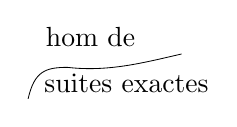
\begin{tikzpicture}[baseline=(base.base)]
\node[anchor=base west,inner sep=0] (base) at (0,0) {suites exactes};
\node[anchor=base west,inner sep=0] at (.02,.58) {\inserted{hom de}};
\draw[line width=.3pt] (-.20,-.08) .. controls (-.12,.27) and (.02,.32) .. (.30,.32) .. controls (.82,.26) and (1.27,.38) .. (1.75,.49);
\end{tikzpicture}
\margin{sauf si $g=0,\nu=0,1,2$\quad\figure{\begin{tikzpicture}\node[draw,ellipse] {$g=1,\nu=0$};\end{tikzpicture}}?}
\diagram{(4)\quad\begin{tikzcd}[ampersand replacement=\&,column sep=small,row sep=large]
1 \arrow[r,dash] \& \pi_1(\overline M_{g,\nu};\unsure{\xi|j}) \arrow[r,dash] \arrow[d,"\tikz[baseline=-.5ex]{\node[rotate=90,inner sep=0pt] {$\approx$};}"',"\deleted{\unsure{\mathcal T_{g\nu}^{\wedge}}}"] \& \pi_1(M_{g,\nu};\unsure{\xi|j}) \arrow[r] \arrow[d] \& \Gamma \arrow[r,dash] \arrow[d,bend left=20] \& 1\\
1 \arrow[r] \& \mathcal T_{g,\nu}^{\wedge} \arrow[r] \& \operatorname{Autextlac}^{\circ}(\pi_1(X_{\unsure{\xi|j}}\setminus\{x_1,-x_\nu)) \arrow[r] \& \operatorname{Out}\unsure{T} \arrow[d,phantom,"\unsure{\vert|\downarrow}" description]\\
\&\&\&1
\end{tikzcd}}
\unsure{admettons} que $\mathcal T_{g,\nu}^{\wedge}\unsure{\to|\text{est}}$
\unsure{invariant|injective} dans $\operatorname{Autextlac}^{\circ}(\ ?\ )$.
\margin{Version corrigée éventuelle : $\pi_1(M_{g,\nu};\unsure{\xi|j})\simeq$ Normalisateur de $\mathcal T_{g,\nu}^{\wedge}$ dans $\operatorname{Autextlac}^{\circ}(\pi_1(X_{\unsure{\xi|j}}\setminus\{x_1-x_\nu\unsure{\})|\}))}$ induisant des \unsure{autom} de $\mathcal T_{g,\nu}^{\wedge}$ commutant à $\mathfrak S_\nu$ et préservant une structure
\figure{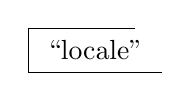
\begin{tikzpicture}
\node[inner sep=1pt] (loc) at (0,0) {``locale''};
\draw (-.85,.28)--(-.85,-.28)--(.85,-.28);
\draw (-.85,.28)--(.5,.28);
\end{tikzpicture}}
éventuelle\ldots $*$
\figure{\begin{tikzpicture}\draw (0,0)--(3.7,0);\end{tikzpicture}}}

On \deleted{\unsure{a}} aimerait que la flèche (1) (la flèche verticale centrale de (5)) soit un \uline{iso}. Cela donnerait une caractérisation de $\Gamma$ comme
\[
\operatorname{Autextlac}^{\circ}\left(\pi_1\underbrace{(X^{an}\setminus\{x_1,-x_\nu\})^{\wedge}}_{\substack{\text{groupe standard}\\\text{bien connu}}}\right)/\mathcal T_{g,\nu}^{\wedge}
\]
\margin{Pour $(g,\nu)$ sauf $g=0,\nu=0,1,2$\quad $g=1,\nu=0$ (cas où $\pi_1(X_{\unsure{\overline{\mathbf Q}|\mathbf Q}}\setminus S_\nu)$ \unsure{est un gr|est un groupe} abélien).
\figure{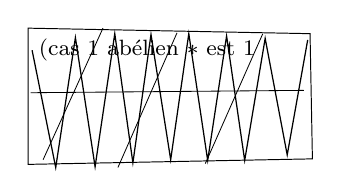
\begin{tikzpicture}
\node[anchor=north west,align=left,text width=3.4cm,font=\footnotesize,inner sep=0] at (0,.85) {\deleted{\unsure{(cas} \illegible{1} \unsure{abélien} $*$ \unsure{est} \illegible{1}}};
\draw[line width=.35pt] (-.13,-.75)--(-.13,.98)--(3.45,.91)--(3.48,-.68)--cycle;
\draw[line width=.45pt] (-.08,.70)--(.22,-.79)--(.47,.86)--(.72,-.78)--(.97,.91)--(1.20,-.73)--(1.43,.90)--(1.68,-.69)--(1.91,.91)--(2.15,-.70)--(2.39,.88)--(2.62,-.70)--(2.88,.85)--(3.16,-.63)--(3.42,.83);
\draw[line width=.3pt] (.06,-.69)--(.82,.98) (1.01,-.79)--(1.76,.92) (2.12,-.74)--(2.85,.91) (-.10,.16)--(3.37,.19);
\end{tikzpicture}}}
\margin{Pour le cas $g=0,\nu=3$, il convient aussi d'être prudent et d'exiger des conditions de commutations avec \unsure{op|op.} ext. de $\mathfrak S_3$\ldots}

\uline{Ex} Pour $g=0,\nu=3$ celà donnerait l'expression déjà envisagée de $\Gamma$ comme
\[
\operatorname{Autextlac}^{\circ}(\pi_1(\mathbf P^1\setminus\{0,1,\infty\}).
\]
\mspage{29}
